\documentclass[12pt]{article}
\usepackage[utf8]{inputenc}
\usepackage{geometry}
\usepackage{graphicx}
\usepackage{xcolor}
\usepackage{titlesec}
\usepackage{multicol}
\usepackage{float}

\geometry{a4paper, margin=1in}

\titleformat{\section}
  {\normalfont\Large\bfseries\color{orange}}
  {\thesection}{1em}{}

\titleformat{\subsection}
  {\normalfont\large\bfseries\color{brown}}
  {\thesubsection}{1em}{}

\begin{document}

\title{\textcolor{orange}{\Huge Vegan Chocolate-Swirled Pumpkin Bundt Cake}}
\author{Adapted from Diane Forley of Flourish Baking Company and Meringueshop}
\date{}

\maketitle

\begin{multicols}{2}

% Added image here
\begin{figure}[H]
\centering
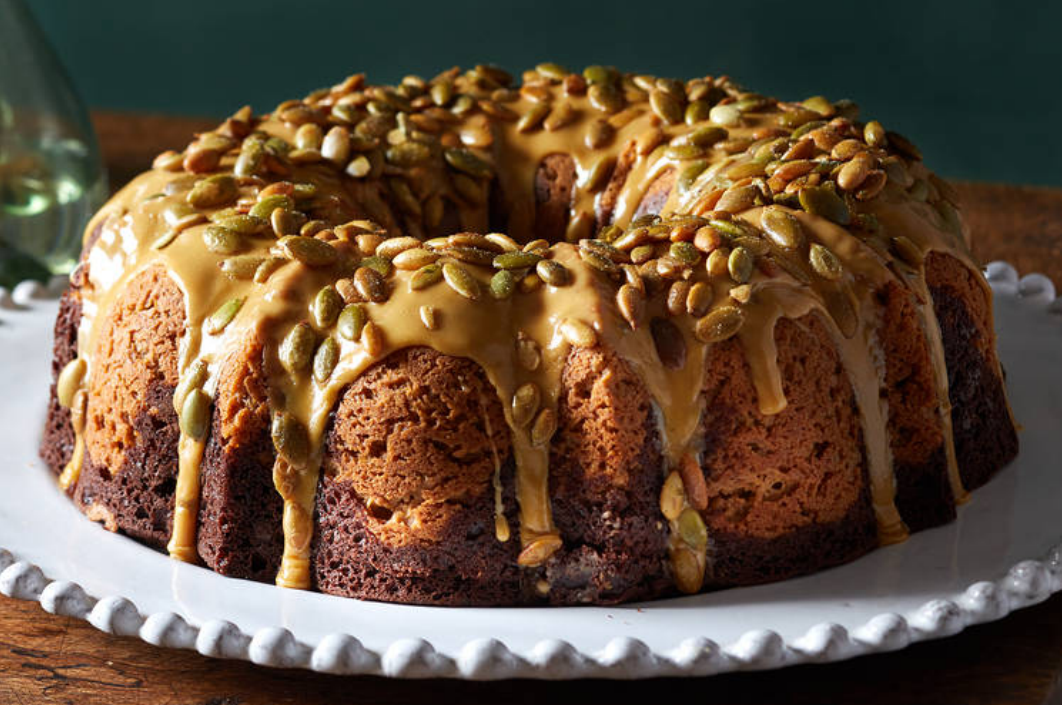
\includegraphics[width=\columnwidth]{bundt.png}
\caption{Vegan Chocolate-Swirled Pumpkin Bundt Cake}
\end{figure}

\section{Ingredients}

\subsection{For the cake:}
\begin{itemize}
    \item ½ cup sunflower seed oil, plus more for greasing pan
    \item 2 cups all-purpose flour, plus more for dusting
    \item 1 cup plus 2 tablespoons rice milk, oat milk, or preferred plant-based milk
    \item 1 tablespoon apple cider vinegar, or distilled white vinegar
    \item 1½ teaspoon baking powder
    \item 1½ teaspoon baking soda
    \item ½ teaspoon salt
    \item 2¼ cups granulated sugar
    \item 1/3 cup maple syrup or brown rice syrup
    \item 2 cups (15-oz can) unsweetened pumpkin puree (without spices)
    \item 2 teaspoons vanilla extract
    \item ½ cup cocoa powder
    \item 1 teaspoon ground cinnamon
    \item ¼ teaspoon ground nutmeg
    \item ¼ teaspoon ground allspice
    \item Salted pepitas, for garnish
\end{itemize}

\subsection{For the glaze:}
\begin{itemize}
    \item 2 cups powdered sugar
    \item 1 tablespoon molasses, or maple syrup
    \item 3 tablespoons rice milk, oat milk or preferred plant-based milk
\end{itemize}
\end{multicols}

\newpage

\section{Instructions}

\begin{enumerate}
    \item Preheat oven to 350°F (175°C). Lightly oil a 10-to-12-quart Bundt pan or 3-pound (4-by-2-by-9-inch) loaf pan. Dust with flour and tap out excess. Set aside.
    
    \item In a small bowl, combine 1 cup rice milk with vinegar and let sit at least 10 minutes. In a medium bowl, sift together flour, baking powder, baking soda and salt.
    
    \item Use an electric mixer fitted with paddle attachment to beat together oil, 2 cups sugar and maple syrup on medium speed until evenly combined, 1 minute. Gradually add pumpkin purée, vanilla extract and rice milk mixture. Continue to beat until ingredients are well incorporated. Turn off mixer. Add dry ingredients and beat on low speed until just combined.
    
    \item Make the chocolate swirl: Transfer 1½ cups batter to another bowl. Add cocoa powder, remaining sugar and remaining rice milk, and whisk until smooth.
    
    \item Add cinnamon, nutmeg and allspice to batter in mixer and beat on low speed to incorporate.
    
    \item Pour batters into prepared Bundt pan in alternating layers, 1 cup pumpkin batter followed by ½ cup chocolate batter. Repeat until you use up batters. Bake until a skewer inserted in cake comes out clean, about 1½ hours. Let cake cool in pan on a baking rack 20 minutes before removing.
    
    \item Make the glaze: In a medium bowl, whisk together powdered sugar, molasses and rice milk to combine. Add more powdered sugar to adjust thickness of glaze as necessary. For a stiffer icing, use a stand mixer with a paddle attachment and beat on high speed until lightened in color, 5 minutes.
    
    \item Place wax paper beneath cooling rack. Turn cake out of Bundt pan onto cooling rack. Spoon glaze over surface of cake to coat. While glaze is still wet, sprinkle a few handfuls of pumpkin seeds all over. You may need to gently press them into the cake to help them adhere.
\end{enumerate}

\textit{Active Time: 40 minutes | Total Time: 2¼ hours | Serves: 8-10}

\end{document}